
%% This file represents a sample first chapter of the main body of the dissertation
%%
%%**********************************************************************
%% Legal Notice:
%% This code is offered as-is without any warranty either
%% expressed or implied; without even the implied warranty of
%% MERCHANTABILITY or FITNESS FOR A PARTICULAR PURPOSE!
%% User assumes all risk.
%% In no event shall any contributor to this code be liable for any damages
%% or losses, including, but not limited to, incidental, consequential, or
%% any other damages, resulting from the use or misuse of any information
%% contained here.
%%**********************************************************************
%%
%% $Id: chapterOne.tex,v 1.6 2006/08/24 21:13:45 Owner Exp $
%%

% A first, optional argument in [ ] is the title as displayed in the table of contents
% The second argument is the title as displayed here.  Use \\ as appropriate in
%   this title to get desired line breaks
\chapter[Introduction]{Introduction}

\section{Background}

\subsection{Magnetosphere}

\subsubsection{Discovery}
The dynamic processes of Earth's magnetosphere and their various impacts on the planet and its inhabitants have been studied for centuries: from Celsius and Hiorter who noted a correlation between compass orientation and aurora \cite{Maunder}, and the Carrington event in 1859 established the connection between solar output and electromagnetic effects on Earth \cite{Carrington}. 

It wasn't until Van Allen did his rocket sounding and satellite measurements of high altitude cosmic rays, finding the eponymous Van Allen Radiation Belt, that the structure of the magnetosphere was generally accepted to be more complex than that of a basic dipole magnet \cite{MagnetoHistory}. Showing that charged particles in solar wind plasma could be broken into constituent parts and directed into currents led to a deeper understanding of the behavior the magnetosphere and its interconnectivity with structures both inwards and outwards, which in turn allowed for better forecasting of ground-based effects based on solar wind conditions.

Our current computational technology, combined with over 50 years' worth of satellite and ground based measurements \cite{HistMagnetometer}, allows for a much stronger statistics-based forecasting method to be performed and long-term analyses of the capabilities of computationally intensive forecasting methods.


\subsubsection{Processes}

The complex structure of the magnetosphere and plasmasphere lead to a number of distinct behaviors and processes such as ring currents, geomagnetic storms, and magnetospheric substorms.

\paragraph{Ring Current}
The Ring Current, shown in Figure \ref{RingCurrentFigure} is a formed when the magnetosphere splits the neutral solar wind into positive and negative components, where they circle the earth moving along magnetic field lines until they either connect with particles in the upper atmosphere/ionosphere and fall out, or remain trapped in the magnetosphere and slowly drift in opposing directions around the magnetic equator. With enough energetic particles drifting together, a current is generated that can significantly affect the Earth's magnetic field and is labeled the Ring Current. These particles in the current are injected into the magnetosphere via conditions that cause the solar wind's magnetic field to connect with that of Earth, which is often exacerbated by the surge of energy created by geomagnetic storms.

\begin{figure}[htp]
\centering
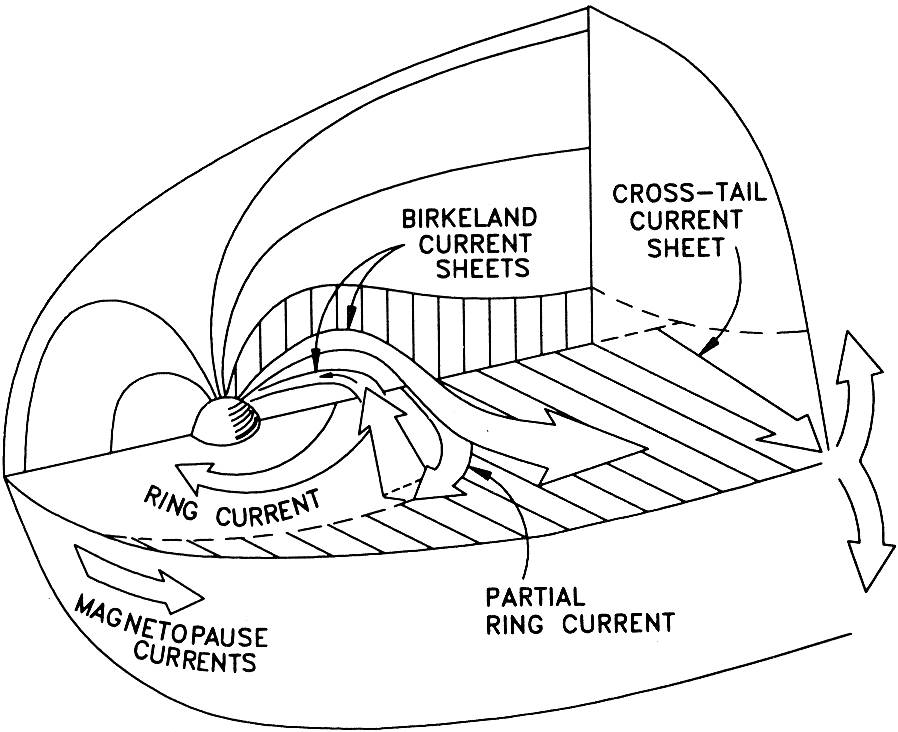
\includegraphics[scale=0.80]{{Figures/MagnetosphereCurrents.jpg}}
\caption{Currents in/around the magnetosphere \cite{RingCurrentMapping}}
\label{RingCurrentFigure}
\end{figure}


Geomagnetic storms occur when the solar wind interacts with the Earth's magnetosphere in such a way as to produce significant disruptions in its normal, quiet-time, behavior. It is generally defined by a significant change to the magnetic field measured by multiple ground-based magnetometer measurements from stations spread around the world, in the case of the $K_P$ index, or around the geomagnetic equator in the case of the Disturbance storm-time ($D_{st}$) index. By using these indices, storms can be classified into categories of severity \cite{NOAAScale}. The definition of storms in the literature varies slightly between authors \cite{Yermolaev}, but most agree that sustained and abnormally perturbed near-earth magnetic field strengths over several hours or more constitutes a geomagnetic storm \cite{StormDefinition}. 

Geomagnetic substorms, in contrast with storms, are much shorter; typically only existing for an hour or two, and potentially happening soon after one another. They tend to have a less appreciable effect on the amount of particles/energy in the ring current, and are associated with sudden changes in energy coming from the tail of the magnetosphere rather than the dayside reconnections associated with storms, and is often directly injected into the polar regions.


Geomagnetic storms and substorms can have significant impacts on Earth and space systems, from inducing currents in large power grids to harming satellite circuitry and onboard data \cite{1989Storm}. Because of the potential damage of such events, any ability to forecast a storm could allow operators to prevent or mitigate problems in their systems. Becuase of the large correlation of CMEs with geomagnetic storms \cite{Yermolaev}, it can be estimated that our forewarning time is the difference between observing a CME (via visual or X-ray methods) and its propagation time plus magnetospheric interaction time. This time can be anywhere from one to five days, depending on the speed of the CME and how it interacts with the interplanetary medium \cite{StormSources}. With a light delay of only eight minutes, this is ample time to see a storm approaching Earth and for operators to react, but a problem lies in the fact that storms are poorly predicted with such lead times \cite{WeigelDecision}. Some storms have slow onsets, some spike suddenly; some have high velocities, and some coincide with large amounts of high-energy particles; no single factor has yet proven to be a good predictor for storms, and while prediction has gradually improved over the years, there remains room for further study. 



Leave off with statement on how outer magnetosphere influences plasmasphere.

\subsection{Plasmasphere}

\subsubsection{Discovery}

\subsubsection{Processes}

Plumes, erosion, etc.

Leave off with list of things that are not well understood and how work in thesis approaches them.

\subsection{Statistical Modeling of Magnetopshere and Plasmasphere}

Initial forecasts were based on an observed time delay between sunspots and geomagnetic storms \cite{SunspotStorms}. It then advanced to a basic theory involving electromagnetic interactions in the magnetosphere \cite{Chapman}. There now exist entire services dedicated to executing MHD-based models of the magnetosphere \cite{CCMC}, as well as multi-year, multi-institution efforts to survey the general statistics of modeling and forecasting of extreme events \cite{ExtremeEvents}.

The convergence of the advancement in both statistical and MHD-based simulation has led to a situation where the scientific community has the capacity for monitoring space weather in real time, and forecasting the near-Earth effects.  There have been efforts to test the forecast performance of select models over a small number of geomagnetic events \cite{ANNforecast,StormModel,StatCompStorms,Yermolaev}. However no research has been done that involves the analysis of long-term forecasting performance of these models and comparison of the results with existing methods.


Make connection to each paper with a section in chapter 2.


